\section{prefetch\_\-nextline\_\-t Class Reference}
\label{classprefetch__nextline__t}\index{prefetch\_\-nextline\_\-t@{prefetch\_\-nextline\_\-t}}
Inheritance diagram for prefetch\_\-nextline\_\-t:\nopagebreak
\begin{figure}[H]
\begin{center}
\leavevmode
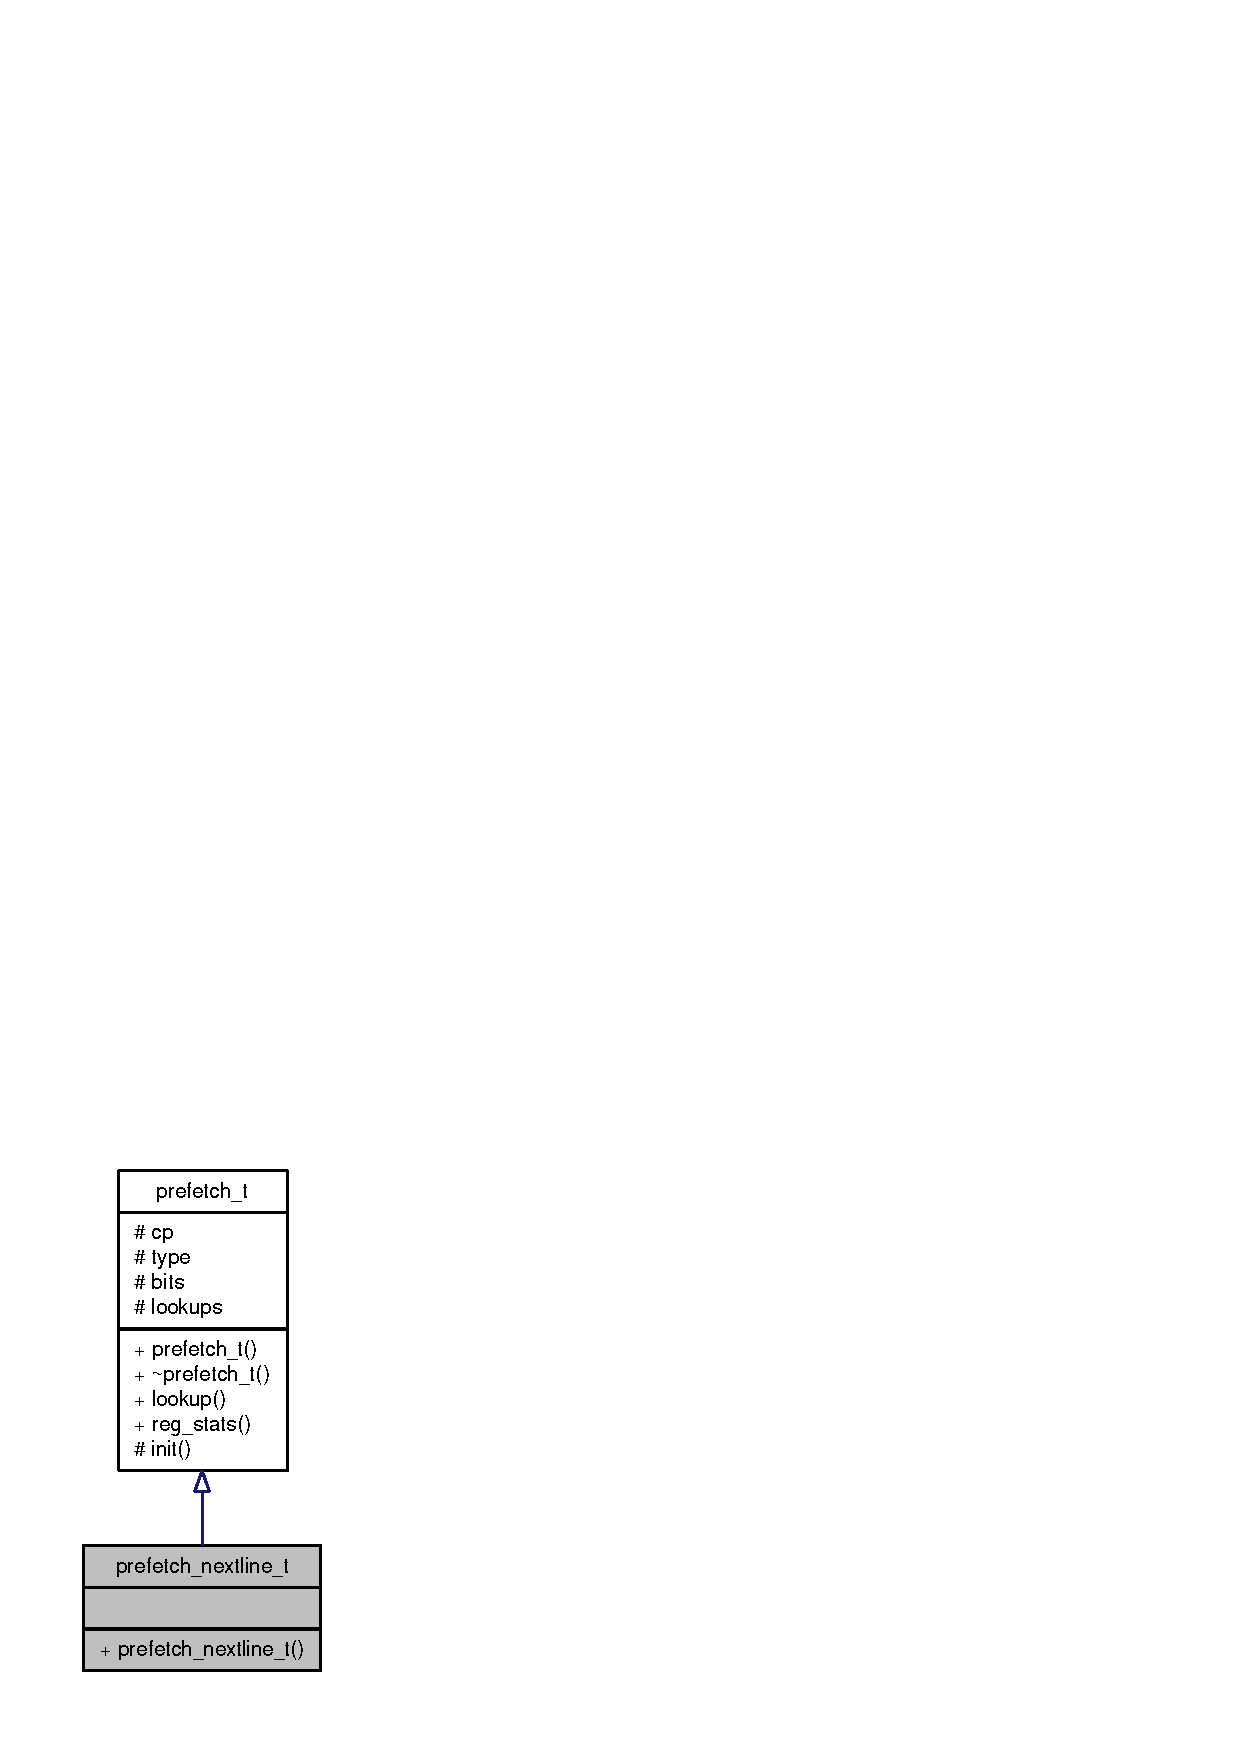
\includegraphics[width=158pt]{classprefetch__nextline__t__inherit__graph}
\end{center}
\end{figure}
Collaboration diagram for prefetch\_\-nextline\_\-t:\nopagebreak
\begin{figure}[H]
\begin{center}
\leavevmode
\includegraphics[width=400pt]{classprefetch__nextline__t__coll__graph}
\end{center}
\end{figure}
\subsection*{Public Member Functions}
\begin{CompactItemize}
\item 
{\bf prefetch\_\-nextline\_\-t} (struct {\bf cache\_\-t} $\ast$arg\_\-cp)
\end{CompactItemize}


\subsection{Detailed Description}


Definition at line 15 of file prefetch-nextline.cpp.

\subsection{Constructor \& Destructor Documentation}
\index{prefetch\_\-nextline\_\-t@{prefetch\_\-nextline\_\-t}!prefetch\_\-nextline\_\-t@{prefetch\_\-nextline\_\-t}}
\index{prefetch\_\-nextline\_\-t@{prefetch\_\-nextline\_\-t}!prefetch_nextline_t@{prefetch\_\-nextline\_\-t}}
\subsubsection[{prefetch\_\-nextline\_\-t}]{\setlength{\rightskip}{0pt plus 5cm}prefetch\_\-nextline\_\-t::prefetch\_\-nextline\_\-t (struct {\bf cache\_\-t} $\ast$ {\em arg\_\-cp})\hspace{0.3cm}{\tt  [inline]}}\label{classprefetch__nextline__t_6363ced0b7a39b024c645e376becc967}




Definition at line 19 of file prefetch-nextline.cpp.

References prefetch\_\-t::bits, prefetch\_\-t::cp, fatal(), prefetch\_\-t::init(), and prefetch\_\-t::type.

The documentation for this class was generated from the following file:\begin{CompactItemize}
\item 
{\bf prefetch-nextline.cpp}\end{CompactItemize}
